\documentclass[final]{article}

\usepackage[paperwidth=84.1cm,paperheight=118.9cm,margin=2.4cm]{geometry}
\usepackage{graphicx}
\usepackage{xcolor}
\usepackage{tcolorbox}
\usepackage{tikz}
\usepackage{parskip}
\usepackage{mathtools}
\usepackage[style=english]{csquotes}
\usepackage{lmodern}

\usepackage{amsmath, amssymb}
\usepackage{enumitem}

\pagestyle{empty}
\renewcommand{\familydefault}{\sfdefault}
\graphicspath{{LaTeX/images/}{Abschlussarbeit_2021/LaTeX/images/}{Images/}}

\definecolor{posterline}{RGB}{220,220,220}
\definecolor{posteraccent}{RGB}{0,104,125}

\newcommand{\postertitle}{Spectral Scale Selection in Topological Data Analysis}
\newcommand{\posterauthor}{Ilja Sukhanov\textsuperscript{1} \quad Djordje Baralic\textsuperscript{2} \quad Oleksandr Leonov\textsuperscript{3} \quad Liudmyla Polyakova\textsuperscript{3} \quad Evgeny Spodarev\textsuperscript{1}}
\newcommand{\posterinfo}{\textsuperscript{1} Universität Ulm, Germany \quad \textsuperscript{2} MISANU, Belgrade \quad \textsuperscript{3} Kharazin National University, Charkiw}

\setlength{\parskip}{0.48em}
\setlist[itemize]{leftmargin=1.1em,itemsep=0.1em,topsep=0.1em}
\setlist[enumerate]{leftmargin=1.4em,itemsep=0.3em,topsep=0.3em}

\tcbset{
  posterblockstyle/.style={
    colback=white,
    colframe=black!55,
    colbacktitle=white,
    coltitle=black,
    fonttitle=\fontsize{24}{29}\selectfont\bfseries,
    fontupper=\fontsize{17}{21.8}\selectfont,
    boxrule=1.1pt,
    arc=0pt,
    left=0.7cm,
    right=0.7cm,
    top=0.62cm,
    bottom=0.72cm,
  }
}

\newcommand{\posterblock}[2]{%
  \begin{tcolorbox}[posterblockstyle,title={#1}]
    #2
  \end{tcolorbox}
  \vspace{0.95cm}
}
\newcommand{\posterequation}[1]{%
  \par\smallskip
  \begin{center}
    \setlength{\fboxsep}{0.32cm}%
    \setlength{\fboxrule}{0.7pt}%
    \fcolorbox{black!35}{black!4}{$\displaystyle #1$}%
  \end{center}
  \smallskip
}
\newcommand{\posterequationbox}[1]{%
  \setlength{\fboxsep}{0.32cm}%
  \setlength{\fboxrule}{0.7pt}%
  \fcolorbox{black!35}{black!4}{$\displaystyle #1$}%
}
\newcommand{\posterequationpair}[4]{%
  \par\smallskip
  \noindent\makebox[\linewidth][c]{%
    \begin{minipage}[c]{#1\linewidth}
      \centering\posterequationbox{#3}%
    \end{minipage}%
    \hspace{0.5em}%
    \begin{minipage}[c]{#2\linewidth}
      \centering\posterequationbox{#4}%
    \end{minipage}%
  }%
  \par\smallskip
}
\newcommand{\posterimageframe}[2]{%
  \begingroup
  \setlength{\fboxsep}{0pt}%
  \makebox[\linewidth][c]{%
    \fcolorbox{posterline}{white}{%
      \parbox[t][#1][t]{0.98\linewidth}{%
        \vspace{0pt}\centering
        \includegraphics[width=\linewidth,height=#1,keepaspectratio]{#2}%
      }%
    }%
  }%
  \endgroup
}
\newcommand{\postercenteredimageframe}[2]{%
  \begingroup
  \setlength{\fboxsep}{0pt}%
  \makebox[\linewidth][c]{%
    \fcolorbox{posterline}{white}{%
      \parbox[c][#1][c]{0.98\linewidth}{%
        \centering
        \includegraphics[width=\linewidth,height=#1,keepaspectratio]{#2}%
      }%
    }%
  }%
  \endgroup
}
\newcommand{\posterreferences}{%
  \begin{tcolorbox}[
    posterblockstyle,
    title={References},
    fonttitle=\fontsize{20}{24}\selectfont\bfseries,
    fontupper=\fontsize{13}{16}\selectfont
  ]
    \textbf{[1]} M. Schlather. \emph{An Algebraic Generalization of the Entropy and Its Application to Statistics}. arXiv:2404.05854, 2024.\par\smallskip
    \textbf{[2]} F. Chazal and B. Michel. \emph{Covers and Nerves: Union of Balls, Geometric Inference and Mapper}. Introduction to Topological Data Analysis, Barcelona, 2016.\par\smallskip
    \textbf{[3]} S. Glushakov, I. Kotenko, and K. Drach. \emph{Understanding the Spread of COVID-19 in the United States Using Topology and Machine Learning for Time Series}. PHUSE EU Connect, 2020.\par\smallskip
    \textbf{[4]} M. Girvan and M. E. J. Newman. \emph{Community structure in social and biological networks}. Proceedings of the National Academy of Sciences 99(12), 7821--7826, 2002.
  \end{tcolorbox}
}
\begin{document}
\begin{tikzpicture}[remember picture,overlay]
  \draw[posterline,line width=1.5pt]
    ([xshift=2.4cm,yshift=-9.4cm]current page.north west) --
    ([xshift=-2.4cm,yshift=-9.4cm]current page.north east);
\end{tikzpicture}

\begin{minipage}[t]{0.68\textwidth}
  {\fontsize{46}{53}\selectfont\bfseries\postertitle\par}
  \vspace{0.65cm}
  {\fontsize{21}{26}\selectfont\posterauthor\par}
  \vspace{0.28cm}
  {\fontsize{17}{21}\selectfont\posterinfo\par}
\end{minipage}
\hfill
\begin{minipage}[t]{0.24\textwidth}
  \raggedleft
  
\includegraphics[width=0.85\linewidth]{logo_uulm_sw.png}
\end{minipage}

\vspace{1.3cm}
\enlargethispage{5cm}

\begin{minipage}[t]{0.48\textwidth}
\vspace{0pt}
    \posterblock{1. Why Select One Scale}{
    \begin{itemize}
        \item Persistent homology is scale-agnostic: persistence diagrams record features \textbf{across all filtration scales}.
        \item Nevertheless, many problems in and around TDA reduce to the \textbf{choice of one filtration parameter}.
        \item This choice should be made in a \textbf{theoretically justified} way.
    \end{itemize}

    \vspace{0.6em}

    \begin{center}
    \setlength{\fboxsep}{6pt}
    \renewcommand{\arraystretch}{1.4}
    \begin{tabular}{cc}
        \fbox{
            \begin{minipage}{0.42\linewidth}
                \centering
                \textbf{Reconstruction and meshing from point clouds}
            \end{minipage}
        }
        &
        \fbox{
            \begin{minipage}{0.42\linewidth}
                \centering
                \textbf{Topology-aware clustering and graph construction}
            \end{minipage}
        }
        \\[0.8em]
        \fbox{
            \begin{minipage}{0.42\linewidth}
                \centering
                \textbf{Statistical inference for point processes}
            \end{minipage}
        }
        &
        \fbox{
            \begin{minipage}{0.42\linewidth}
                \centering
                \textbf{Materials and physical systems with intrinsic length scales}
            \end{minipage}
        }
    \end{tabular}
    \end{center}
}

\vspace{-0.45cm}

\posterblock{2. Spectral Scale Selection}{
\begin{itemize}
    \item Let $K_1,\dots,K_N$ be simplicial complexes on a common vertex set $X$ and $\oplus$ a commutative binary operation; below, $\oplus=\cup$.
    \item The functional $f$ combines topological or combinatorial features and is \textbf{subadditive} with respect to $\oplus$.
\end{itemize}
Motivated by \textbf{[1]}, define the \textbf{$f$-based divergence} and the \textbf{scale similarity matrix}:
\posterequationpair{0.58}{0.39}
  {\langle K_i,K_j\rangle_f\coloneqq f(K_i)+f(K_j)-f(K_i\oplus K_j),}
  {\Sigma_N\coloneqq \bigl(\langle K_i,K_j\rangle_f\bigr)_{i,j=1}^{N}\in\mathbb{R}^{N\times N}.}

    For a filtration $K_i=\operatorname{VR}_{\epsilon_i}(X)$ with
    $0<\epsilon_1<\cdots<\epsilon_N$,
    \[
        \langle K_i,K_j\rangle_f=f(K_{\min\{i,j\}}),
    \]
    so $\Sigma_N$ is a classical \textbf{min/meet-matrix}:
    \posterequation{
        \begin{aligned}
            \Sigma_N=\begin{pmatrix}
                f(K_1) & f(K_1) & \cdots & f(K_1)\\
                f(K_1) & f(K_2) & \cdots & f(K_2)\\
                \vdots & \vdots & \ddots & \vdots\\
                f(K_1) & f(K_2) & \cdots & f(K_N)
            \end{pmatrix}
        \end{aligned}
    }
    \begin{itemize}
        \item Along the filtration, nonnegativity of $f$ already implies subadditivity.
        \item The matrix $\Sigma_N$ is irreducible iff $f(K_1)>0$.
        \item By \textbf{Perron-Frobenius}, the principal eigenvector $v^*$ is positive and unique up to scaling; it ranks the scales $\epsilon_i$ through their coupling in $\Sigma_N$.
    \end{itemize}
}

\vspace{-0.45cm}

\posterblock{3. Non-monotone Scale Selection}{
    The critical scale is chosen by the rule
    \posterequation{
        \begin{aligned}
            i_{\text{crit}}\in\arg\max_iv^*_i, \quad\epsilon_{\text{crit}}=\epsilon_{i_{\text{crit}}}
        \end{aligned}
    }
    \begin{itemize}
        \item $f(K_i)$ and $v_i^*$ have the same local monotonicity pattern:
        $\operatorname{sgn}(v_{i+1}^*-v_i^*)=\operatorname{sgn}(f(K_{i+1})-f(K_i))$.
        \item Thus, their \textbf{local maxima coincide}.
        \item For non-monotone $f$, global maxima need not coincide and the Perron vector can serve as a \textbf{tiebreaker} between separated equal maxima.
        \item For strictly monotone $f$, the Perron vector reflects the monotonicity and the critical scale lies at an endpoint.
    \end{itemize}

    \vspace{0.5em}

    \begin{center}
        
        \begin{minipage}[t]{0.72\linewidth}
            \vspace{0pt}
            \centering
            \makebox[\linewidth][c]{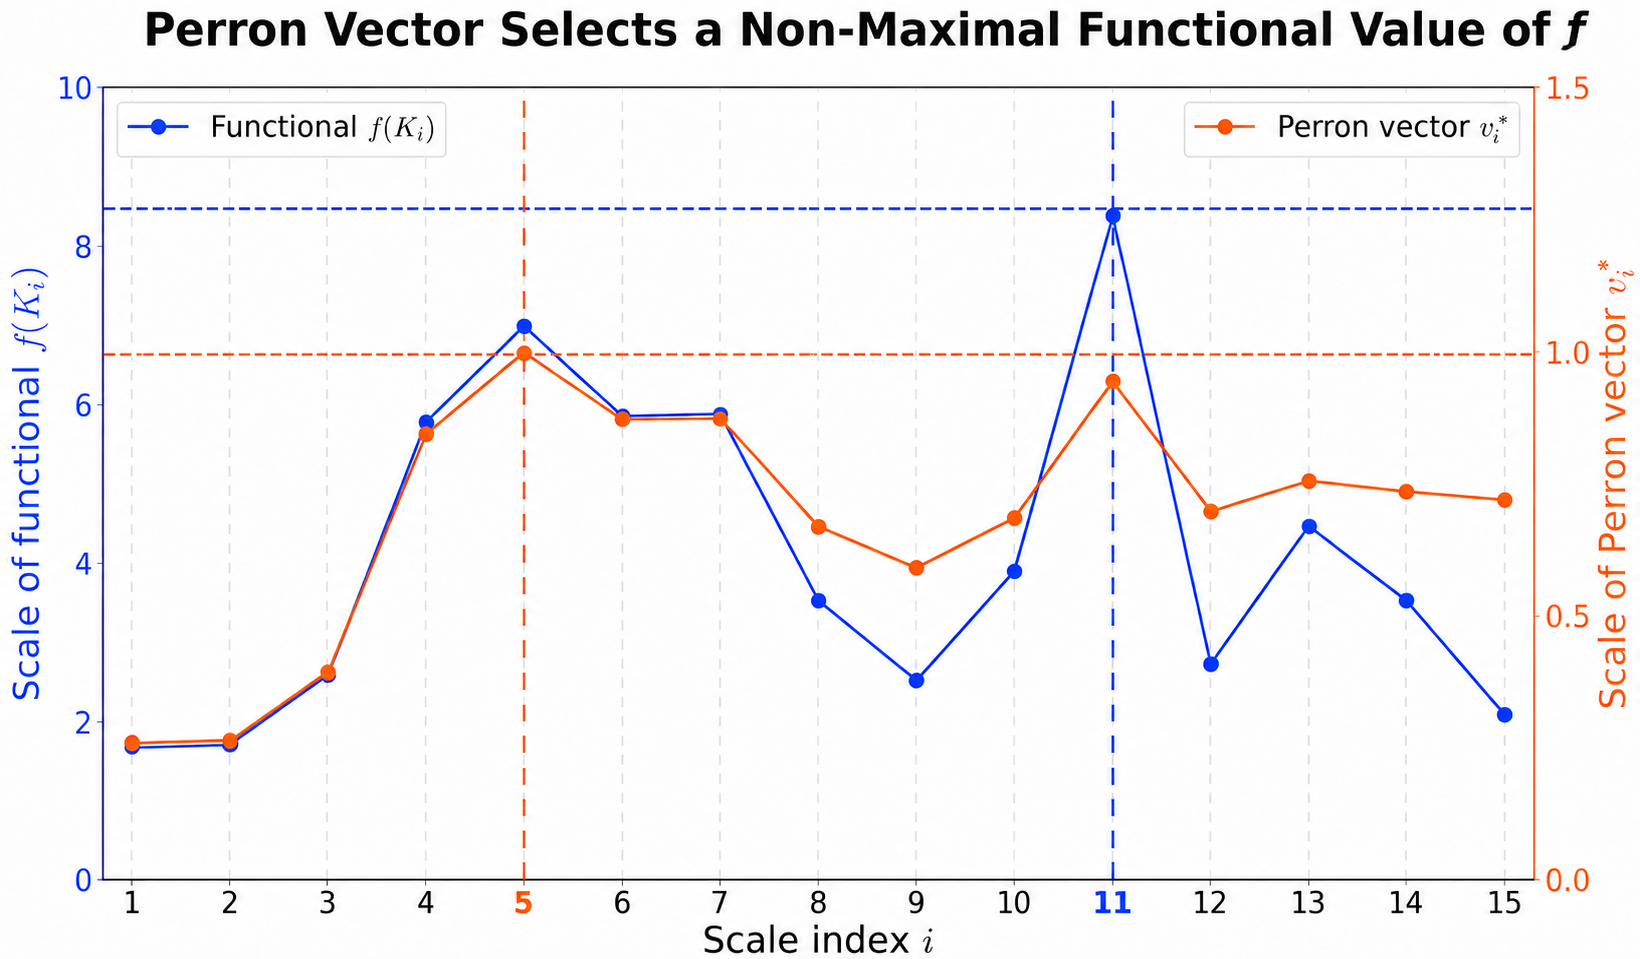
\includegraphics[width=\linewidth]{Abschlussarbeit_2021/LaTeX/images/Functional scale choice 3.png}}

        \end{minipage}

        \vspace{0.55em}

        \begin{minipage}[t]{0.72\linewidth}
            \vspace{0pt}
            \centering
            \makebox[\linewidth][c]{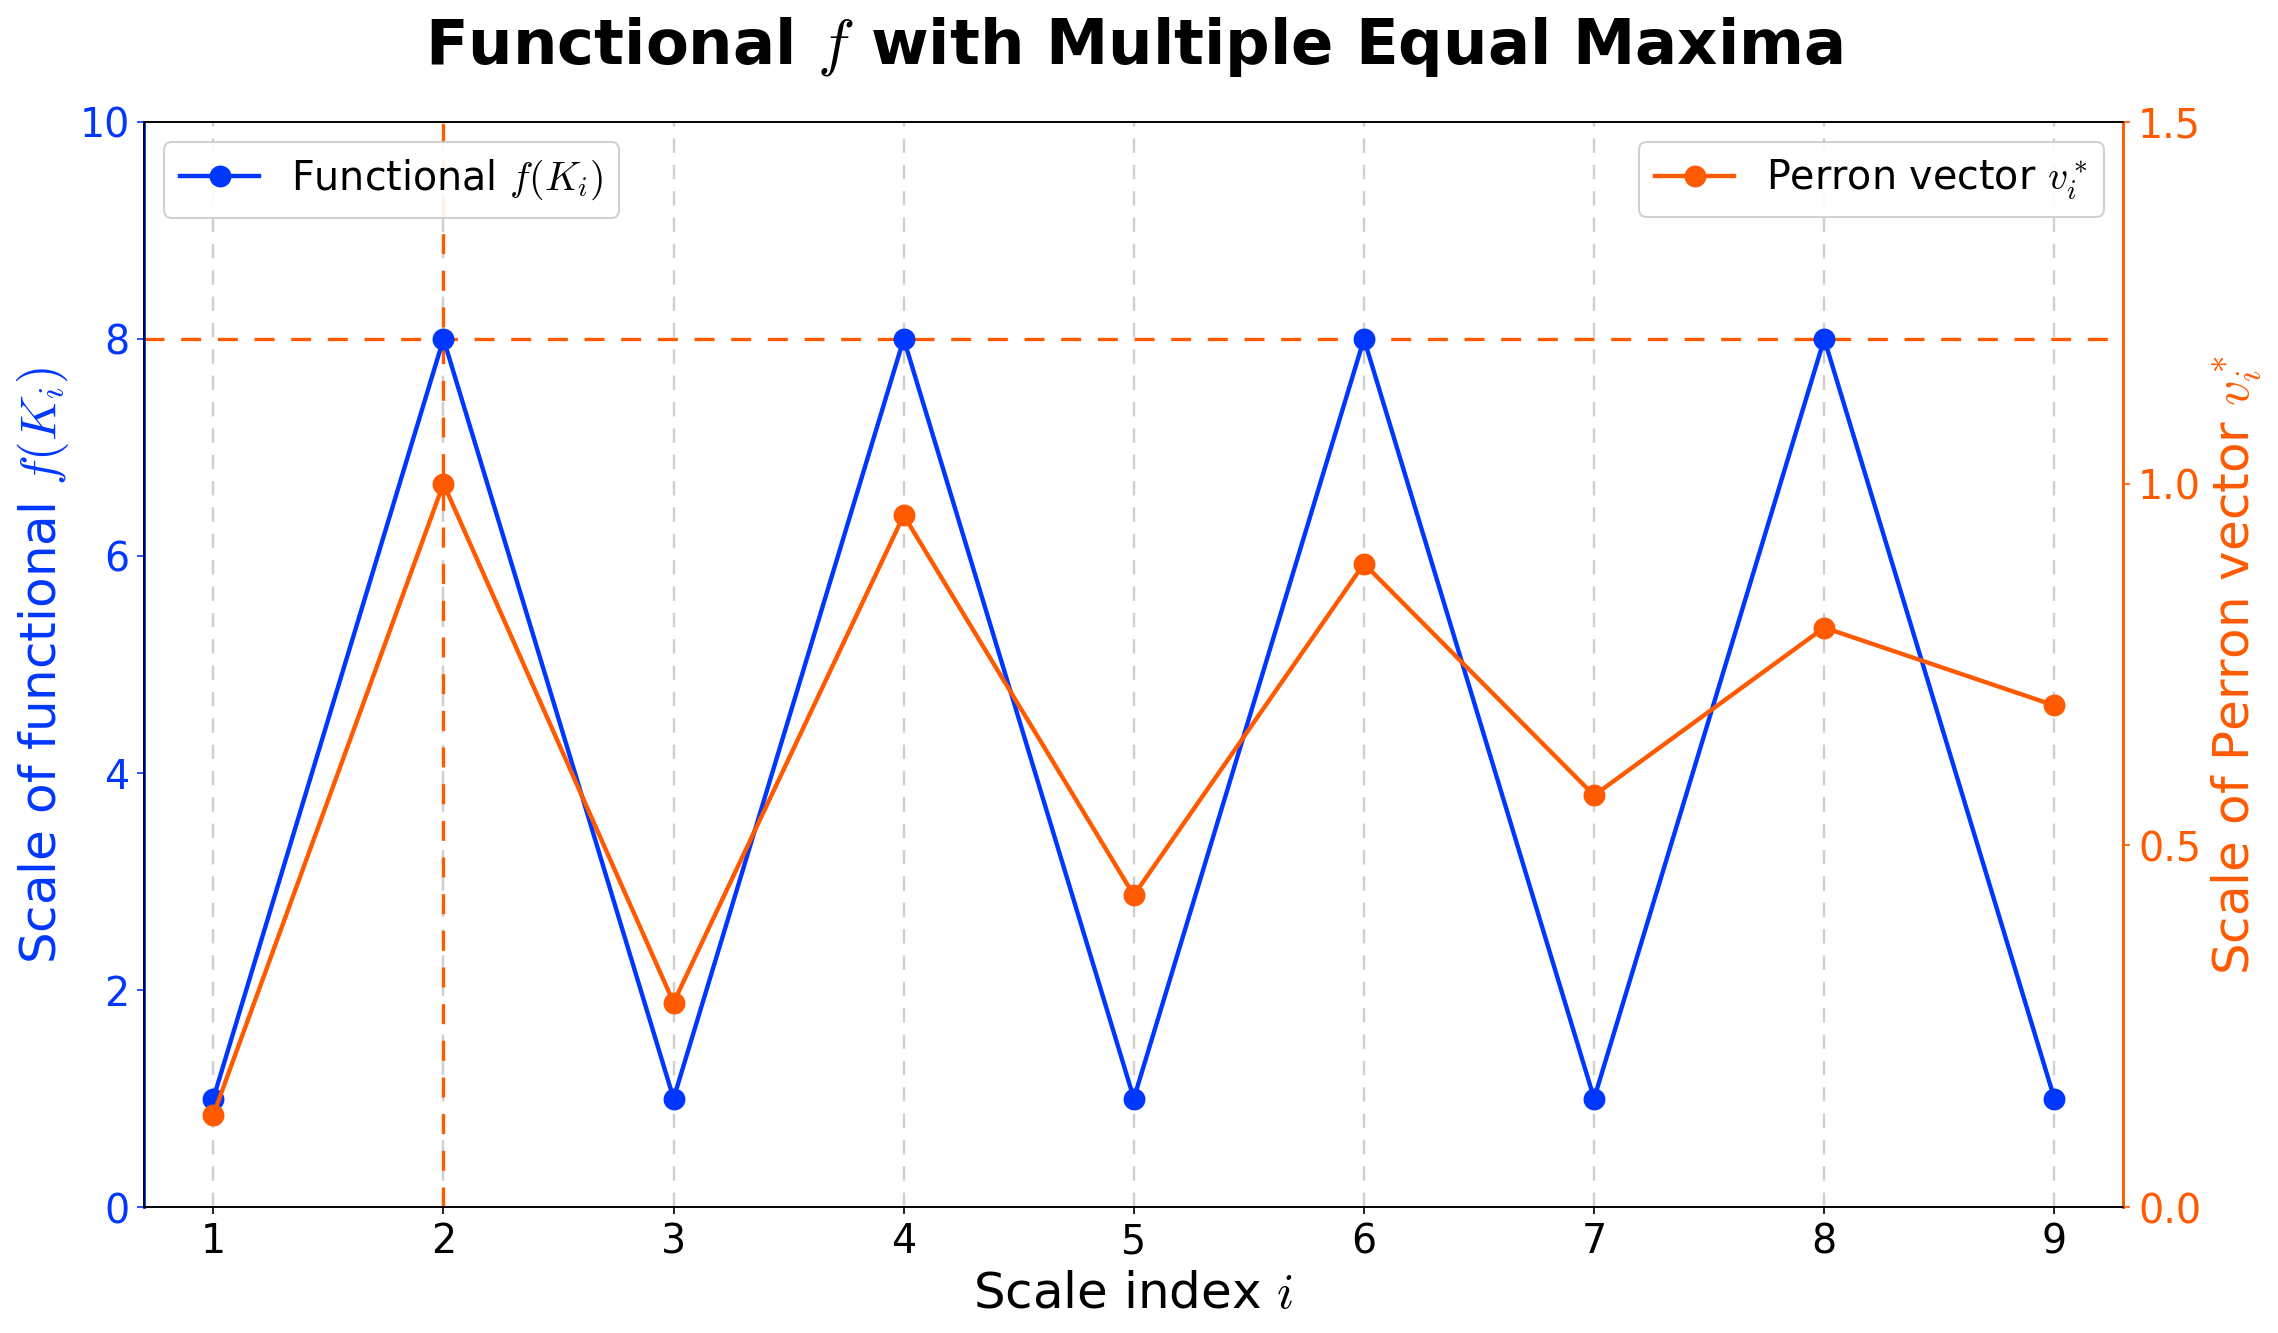
\includegraphics[width=\linewidth]{Abschlussarbeit_2021/LaTeX/images/Functional with multiple equal maxima 3.png}}

        \end{minipage}

    \end{center}

}


\vspace{-0.45cm}

\posterblock{4. Connection to Markov Chains}{
    \begin{itemize}
        \item Associate a \textbf{finite Markov chain} with the scale similarity matrix $\Sigma_N$.
        \item Construct its transition matrix $P$ using \textbf{Doob's $h$-Transform}.
        \item Its stationary distribution is proportional to the squared coordinates of $v^*$:
    \end{itemize}
    \posterequationpair{0.56}{0.39}
      {P=\frac{1}{\lambda^*}D_{v^*}^{-1}\Sigma_ND_{v^*},}
      {\pi_i^{P}=\frac{(v_i^*)^2}{\|v^*\|_2^2},}
    Here $D_{v^*}=\operatorname{diag}(v_1^*,\dots,v_N^*)$. The matrix $P$ maximizes the \textbf{Donsker-Varadhan free-energy functional} over irreducible, row-stochastic matrices:
    \posterequationpair{0.57}{0.40}
      {\mathcal{F}(Q;\Sigma_N)\coloneqq \sum_{i,j=1}^{N}\pi_i^{Q}q_{ij}\log{\frac{(\Sigma_N)_{ij}}{q_{ij}}},}
      {P=\arg\max\left\{\mathcal{F}(Q;\Sigma_N):
       \substack{Q\in\mathbb{R}^{N\times N}\\
       \text{row-stochastic and irreducible}}\right\}.}
    Thus, $P$ is the \textbf{variationally optimal stochastic normalization} of $\Sigma_N$.
}

\vspace{-0.45cm}

\posterblock{5. Monotone Scale Selection}{
    For a strictly increasing functional, $0<f(K_1)<\cdots<f(K_N)$:
    \begin{itemize}
        \item $\Sigma_N$ is positive definite and $\Sigma_N^{-1}$ is tridiagonal.
        \item The \textbf{discrete Laplacian}
        $\mathcal{L}=f(K_1)^{-1}\operatorname{diag}(1,0,\dots,0)-\Sigma_N^{-1}$
        is the generator of a continuous-time birth-death chain on $\{1,\dots,N\}$.
    \end{itemize}
\posterequationpair{0.72}{0.25}
{
\begin{aligned}
\mathcal{L}
&=
\begin{pmatrix}
-\frac{1}{d_2}
&
\frac{1}{d_2}
&
0
&
\cdots
&
0
&
0
\\[0.4em]
\frac{1}{d_2}
&
-\left(\frac{1}{d_2}+\frac{1}{d_3}\right)
&
\frac{1}{d_3}
&
\ddots
&
\vdots
&
\vdots
\\[0.4em]
0
&
\frac{1}{d_3}
&
-\left(\frac{1}{d_3}+\frac{1}{d_4}\right)
&
\ddots
&
0
&
0
\\[0.4em]
\vdots
&
\ddots
&
\ddots
&
\ddots
&
\frac{1}{d_{N-1}}
&
0
\\[0.4em]
0
&
\cdots
&
0
&
\frac{1}{d_{N-1}}
&
-\left(\frac{1}{d_{N-1}}+\frac{1}{d_N}\right)
&
\frac{1}{d_N}
\\[0.4em]
0
&
\cdots
&
0
&
0
&
\frac{1}{d_N}
&
-\frac{1}{d_N}
\end{pmatrix},
\end{aligned}
}
{
\begin{gathered}
d_i=f(K_i)-f(K_{i-1})\\
i=2,\dots,N.
\end{gathered}
}

    For the embedded discrete-time chain,
    $P^{\text{BD}}_{ij}=-(1-\delta_{ij})\mathcal{L}_{ij}/\mathcal{L}_{ii}$.
    Its stationary distribution gives the scale selection rule
    \posterequationpair{0.40}{0.51}
      {i_{\text{crit}}\in\arg\min_i\pi_i^{\text{BD}},}
      {\pi_i^{\text{BD}}=\frac{\mathcal{L}_{ii}}{\sum_{j=1}^{N}\mathcal{L}_{jj}}.}
    \begin{itemize}
        \item For $2\le i\le N-1$, $-\mathcal{L}_{ii}=d_i^{-1}+d_{i+1}^{-1}$.
        \item Minimizing $\pi_i^{\text{BD}}$ favors two large consecutive increments.
    \end{itemize}

    \vspace{0.4em}

    \begin{center}
      \begin{minipage}[t]{0.48\linewidth}
        \vspace{0pt}
        \centering
        \posterimageframe{9.2cm}{Abschlussarbeit_2021/LaTeX/images/Strictly increasing functional 2.png}

      \end{minipage}
      \hfill
      \begin{minipage}[t]{0.48\linewidth}
        \vspace{0pt}
        \centering
        \posterimageframe{9.2cm}{Abschlussarbeit_2021/LaTeX/images/stationary distribution.png}

      \end{minipage}
    \end{center}
}


\end{minipage}
\hfill
\begin{minipage}[t]{0.48\textwidth}
\vspace{0pt}

    \posterblock{6. The Mapper Algorithm vs. Multiscale $\alpha$-neighboring (M$\alpha$N) approach}{
    Let $X=\{x_1,\dots,x_n\}\subseteq\mathbb{R}^{D}$ be equipped with a metric $d$:
    \begin{itemize}
        \item choose a \textbf{lens function} $\ell:X\to\mathbb{R}^{m}$, typically $m\in\{1,2\}$;
        \item choose a \textbf{finite open cover} $\mathcal U=\{U_i\}_{i\in I}$ of $\ell(X)$;
        \item form the pullback cover $X_i=\ell^{-1}(U_i)$.
    \end{itemize}

    \begin{center}
            \begin{minipage}[t]{0.47\linewidth}
                \vspace{0pt}
                \textbf{Popular lens choices}
                \begin{itemize}
                    \item density estimate $\rho(x_i)=\frac{1}{nh^D}\sum_j K\!\left(\frac{d(x_i,x_j)}{h}\right)$
                    \item centrality $c(x_i)=\left(n^{-1}\sum_j d(x_i,x_j)^p\right)^{1/p}$
                \end{itemize}
            \end{minipage}
            \hfill
            \begin{minipage}[t]{0.47\linewidth}
                \vspace{0pt}
                \textbf{Popular cover choices}
                \begin{itemize}
                    \item cover in $1D$: overlapping intervals $\{I_j\}_{j=1}^{N}$
                    \item cover in $2D$: rectangles $U_{ij}=I_i^{(1)}\times I_j^{(2)}$
                \end{itemize}
            \end{minipage}
        \end{center}
    
        \begin{center}
            \begin{minipage}[t]{0.48\linewidth}
                \vspace{0pt}
                \centering
                \posterimageframe{10.7cm}{Abschlussarbeit_2021/LaTeX/images/Mapper illustration 3.png}

            \end{minipage}
            \hfill
            \begin{minipage}[t]{0.48\linewidth}
                \vspace{0pt}
                \centering
                \posterimageframe{10.7cm}{Abschlussarbeit_2021/LaTeX/images/M_alpha_N_image3.png}

            \end{minipage}
        \end{center}

        \begin{itemize}
            \item Mapper \textbf{depends on the clustering algorithm} used on each $X_i$.
            \item Each cluster becomes a node; overlapping clusters are connected by an edge.
            \item M$\alpha$N retains each subject as a node and removes clustering from graph construction; community detection may still be applied afterward.
        \end{itemize}
        \textbf{The question becomes: by which rule should two nodes be connected?}
    }

    \vspace{1cm}

    

    \posterblock{7. M$\alpha$N graph approach: Synthetic dataset experiment}{
        Instead of clustering each $X_i$, connect $x,y\in X$ that belong to a common pullback set if and only if
        \posterequation{
            \begin{aligned}
                d(x,y)\le\max\{2\epsilon_i:i\in I,x,y\in X_i\}
            \end{aligned}
        }

        The threshold $\epsilon_i$ is chosen by applying spectral scale selection to $X_i$ using
        \posterequation{
            \begin{aligned}
                f(K)=C(K)\cdot E(K),
            \end{aligned}
        }
        \begin{itemize}
            \item $C(K)$ is the number of connected components and $E(K)$ the number of edges.
            \item Components merge while new edges appear, so the functional may exhibit \textbf{non-monotone} behavior.
            \item The graph \textbf{adapts its scale locally} instead of imposing one global threshold.
            \item First stress test: the \textbf{\enquote{noisy 8}} dataset.
        \end{itemize}

        \begin{center}
            \begin{minipage}[t]{0.36\linewidth}
                \vspace{0pt}
                {\color{posteraccent}\bfseries Noisy input $X$}\par
                \vspace{0.18cm}
                \posterimageframe{10.8cm}{Abschlussarbeit_2021/LaTeX/images/eight_dataset.png}
            \end{minipage}
            \hfill
            \begin{minipage}[t]{0.60\linewidth}
                \vspace{0pt}
                {\color{posteraccent}\bfseries Select the local scales $\epsilon_i$}\par
                \vspace{0.18cm}
                \noindent
                \begin{minipage}[t]{0.485\linewidth}
                    \vspace{0pt}
                    \postercenteredimageframe{10.8cm}{functional.png}
                \end{minipage}
                \hfill
                \begin{minipage}[t]{0.485\linewidth}
                    \vspace{0pt}
                    \postercenteredimageframe{10.8cm}{principal_eigenvector.png}
                \end{minipage}
            \end{minipage}
        \end{center}

        \vspace{0.35cm}
        \begin{center}
            \begin{minipage}[t]{0.35\linewidth}
                \vspace{0pt}
                {\color{posteraccent}\bfseries Grid stability}\par
                \vspace{0.18cm}
                \postercenteredimageframe{11.1cm}{threshold_stability.png}
            \end{minipage}
            \hfill
            \begin{minipage}[t]{0.305\linewidth}
                \vspace{0pt}
                {\color{posteraccent}\bfseries Random thresholds}\par
                \vspace{0.18cm}
                \postercenteredimageframe{11.1cm}{Abschlussarbeit_2021/LaTeX/images/eight_fail.png}
            \end{minipage}
            \hfill
            \begin{minipage}[t]{0.305\linewidth}
                \vspace{0pt}
                {\color{posteraccent}\bfseries Spectral thresholds}\par
                \vspace{0.18cm}
                \postercenteredimageframe{11.1cm}{Abschlussarbeit_2021/LaTeX/images/eight_proper.png}
            \end{minipage}
        \end{center}
    }

    \vspace{1cm}

    \posterblock{8. Case Study: COVID-19 Spread in the USA}{
        \begin{itemize}
            \item Glushakov et al.~\textbf{[3]} constructed a county-level graph to identify similarities in early COVID-19 trajectories.
            \item They revealed four major communities associated with demographic and healthcare variables.
            \item Here, spectral scale selection determines the local M$\alpha$N thresholds automatically using $f(K)=C(K)E(K)$.
        \end{itemize}

        \noindent
        \begin{minipage}[t]{0.48\linewidth}
            \vspace{0pt}
            \textbf{County representation}
            \begin{itemize}
                \item each node $x_i\in\mathbb{R}^{28}$ represents one of $3{,}142$ US counties and county equivalents
                \item first 14 entries: 13 normalized three-day case aggregates and their log-total
                \item second 14 entries: analogous death features
            \end{itemize}
        \end{minipage}
        \hfill
        \begin{minipage}[t]{0.48\linewidth}
            \vspace{0pt}
            \textbf{Lens and cover}
            \begin{itemize}
                \item chosen lens: $\ell(x)=(\rho(x),c(x))$
                \item chosen cover: overlapping rectangles $U_{ij}=I_i^{(1)}\times I_j^{(2)}$
            \end{itemize}
        \end{minipage}

        \vspace{0.35cm}
        \begin{center}
            \textbf{Similarity metric}\par
            Block-wise Euclidean metric on $\mathbb{R}^{14}\times\mathbb{R}^{14}$:
        \end{center}
        \posterequation{
            \begin{aligned}
                d(x_i,x_j)=\|x_i[1\!:\!14]-x_j[1\!:\!14]\|_2+\|x_i[15\!:\!28]-x_j[15\!:\!28]\|_2
            \end{aligned}
        }

        \begin{itemize}
            \item The \textbf{Girvan--Newman algorithm}~\textbf{[4]} yielded four communities.
            \item \textbf{Left:} color indicates the centrality projection $c(x)$; darker colors represent higher values.
            \item \textbf{Right:} four colors indicate the four communities.
        \end{itemize}

        \begin{center}
            \begin{minipage}[t]{0.48\linewidth}
                \vspace{0pt}
                \centering
                \posterimageframe{16cm}{COVID-projections_coloring.png}
            \end{minipage}
            \hfill
            \begin{minipage}[t]{0.48\linewidth}
                \vspace{0pt}
                \centering
                \posterimageframe{16cm}{COVID_Girvan-Newman_4communities.png}
            \end{minipage}
        \end{center}

    \medskip
    
    \noindent

\begin{minipage}[t]{0.31\linewidth}
    \centering
    \colorbox{gray!10}{
    \parbox{0.90\linewidth}{
        \centering
        {\Large\textbf{4}}\\[-0.2em]
        \textbf{major communities}\\[0.25em]
        identified by Girvan--Newman
    }}
\end{minipage}
\hfill
\begin{minipage}[t]{0.31\linewidth}
    \centering
    \colorbox{gray!10}{
    \parbox{0.90\linewidth}{
        \centering
        {\Large\textbf{}}\\[-0.2em]
        \textbf{statistically significant differences}\\[0.25em]
        in several county-level predictors not used to build the graph
    }}
\end{minipage}
\hfill
\begin{minipage}[t]{0.31\linewidth}
    \centering
    \colorbox{gray!10}{
    \parbox{0.90\linewidth}{
        \centering
        {\Large\textbf{}}\\[-0.2em]
        \textbf{spectrally selected thresholds}\\[0.25em]
        without manual tuning
    }}
\end{minipage}

    \medskip
    }

    \vspace{0.8cm}

    \posterreferences

\end{minipage}

\end{document}
